\documentclass{article}

\usepackage{graphicx}
\usepackage{xcolor}
\usepackage{titling}

\usepackage{pdfpages}

\usepackage{minted}
\setminted{bgcolor=black,style=vim, linenos=true, numbersep=5pt, autogobble=true, breaklines=true, breakautoindent=true, python3=true, fontsize=\footnotesize}


\usepackage{tikz}
\usepackage[tikz]{bclogo}

\usepackage[style=numeric]{biblatex}
\usepackage{hyperref}
\addbibresource{references.bib}

\usepackage{fontawesome5}

\usepackage{times}
\usepackage{mathptmx}

\usepackage{geometry}
\geometry{letterpaper, left=20mm, top=20mm, bottom=20mm, right=20mm}


\usepackage{amsmath}
\usepackage{amssymb}
\usepackage{amsthm}

\newtheorem*{theorem}{Théor\`{e}me}
\newtheorem*{definition}{Définition}
\newtheorem*{proposition}{Proposition}
\newtheorem*{corollary}{Corollaire}
\newtheorem*{lemma}{Lemme}
\newtheorem*{example}{Exemple}
\newtheorem*{exercise}{Exercice}
\newtheorem*{remark}{Remarque}
\newtheorem*{problem}{Problème}
\newtheorem*{question}{Question}
\newtheorem*{conjecture}{Conjecture}
\newtheorem*{notation}{Notation}
\newtheorem*{assumption}{Hypothèse}
\newtheorem*{algorithm}{Algorithme}
\newtheorem*{prof}{Preuve}

\title{Une Revue Critique et Praticien sur: \\ `Sorting Algorithms as Special Cases of a Priority Queue Sort'}
\author{ÖZEL, F.}
\date{today}

\PassOptionsToPackage{table}{xcolor}
\begin{document}

    \begin{titlepage}

        \centering

        \includegraphics[width=0.2\textwidth]{Universite-Galatasaray-Logo-PNG.png}\par\vspace{3cm}
        {\huge \thetitle \par}
        \vspace{1cm}
        {\large \textit \theauthor \par}
        \vfill
        {\large Programme de Mathématiques de l'Université de Galatasaray \par MAT 232 - Algorithme et Programmation Avancée \par 4e semestre \today \par}

    \end{titlepage}


    \section*{Préface}

        Cette documentation ; Il contient l'explication et les applications de l'article `Algorithmes de tri comme cas particuliers d'un tri par file d'attente prioritaire', c'est aussi un journal d'un parcours d'apprentissage individuel. De nombreuses explications sur des concepts et des applications informatiques inconnus sont données.

        Parlons de quelques notions qu'il convient de connaître au préalable. Comme le nom du cours l'indique, nous devons savoir ce que signifie algorithme : Un algorithme est une suite finie et non ambiguë d'instructions et d'opérations permettant de résoudre une classe de problèmes. \footnote{La notion de problème peut être vue dans un sens large, il peut s'agir d'une tâche à effectuer, comme trier des objets, assigner des ressources, transmettre des informations, traduire un texte, etc. Il reçoit des données (les entrées), par exemple les objets à trier, la description des ressources à assigner, des besoins à couvrir, un texte à traduire, les informations à transmettre et l'adresse du destinataire, etc., et fournit éventuellement des données (la sortie), par exemple les objets triés, les associations ressource-besoin, un compte-rendu de transmission, la traduction du texte, etc.} Informallement de plus, un algorithme est une procédure de calcul bien définie qui prend une valeur ou un ensemble de valeurs en entrée et produit une valeur ou un ensemble de valeurs en sortie. Un algorithme est donc une séquence d'étapes de calcul qui transforme l'entrée en sortie. \footnote{Cormen, T. H., Leiserson, C. E., Rivest, R. L.,  Stein, C. (2009). Introduction to algorithms. MIT press.}

        Nous pouvons parler de bien d'autres concepts et définitions, mais nous ne devons pas aller au-delà de notre sujet, alors parlons brièvement des algorithmes de tri. Un algorithme de tri est, en informatique ou en mathématiques, un algorithme qui permet d'organiser une collection d'objets selon une relation d'ordre déterminée. Les objets à trier sont des éléments d'un ensemble muni d'un ordre total. Il est par exemple fréquent de trier des entiers selon la relation d'ordre usuelle `est inférieur ou égal à'. Les algorithmes de tri sont utilisés dans de très nombreuses situations. Ils sont en particulier utiles à de nombreux algorithmes plus complexes dont certains algorithmes de recherche, comme la recherche dichotomique. Ils peuvent également servir pour mettre des données sous forme canonique ou les rendre plus lisibles pour l'utilisateur. 

        Une priority queue est une structure de données qui permet de stocker des éléments avec des priorités assignées, et d'accéder à l'élément de plus haute priorité en premier. Cette structure de données est souvent utilisée dans les algorithmes de tri et de recherche. Il existe plusieurs implémentations de priority queue telles que les heaps binomiaux, les heaps de Fibonacci et les heaps binaires. \footnote{Knuth, D. E. (1997). The art of computer programming: sorting and searching (Vol. 3). Addison-Wesley Professional.} \footnote{Williams, J. W. J. (1964). Algorithm 232: Heapsort. Communications of the ACM, 7(6), 347.}

        Un D-ary heap est une structure de données qui est similaire à un binary heap, mais au lieu de stocker deux enfants pour chaque nœud, chaque nœud stocke D'enfants. Les D-ary heaps sont couramment utilisés dans les algorithmes de tri et de recherche, et sont souvent plus efficaces que les binary heaps pour des valeurs de D supérieures à 2. \footnote{Knuth, D. E. (1997). The art of computer programming: sorting and searching (Vol. 3). Addison-Wesley Professional.}

        On pense qu'on se souvient de tous les mots-clés nécessaires, on dit qu'on va examiner plus en détail les concepts qui s'y rapportent, et on passe à la documentation, en supposant que vous connaissiez les mathématiques.

        \newpage

    
    
    \section*{Un Trés Important Rappel: Complexité (de Quicksort)}

            \begin{minted}{Python}
                def quicksort(array):
                    if len(array) < 2:
                        return array
                    else:
                        pivot = array[0]
                        less = [i for i in array[1:] if i <= pivot]
                        greater = [i for i in array[1:] if i > pivot]
                        return quicksort(less) + [pivot] + quicksort(greater)
            \end{minted}
            
            \subsection*{Worst-Case}
            La taille du tableau est prise comme $n-1$ lorsque le pivot est le plus grand ou le plus petit, ou lorsque tous les éléments sont égaux. C'est la pire situation attendue. 
            Si cela se produit, chaque appel récursif invoque un tableau avec un élément manquant dans la liste précédente. En conséquence, nous effectuons $n$ appels imbriqués d'une liste de longueur $n$ vers une liste à un élément. Cela crée une chaîne de $n-1$ boules de long. $O(n-1)$ commence à s'exécuter.
            Par consequent $$\sum_{i=0}^{n}(n-i) = O(n^2)  $$

            \subsection*{Best-Case}
            Nous obtenons le meilleur des cas si nous pouvons diviser la liste en deux parties égales à chaque fois que nous effectuons l'opération de division. Cela signifie qu'une liste de demi-longueur est traitée à chaque récursivité. Cela signifie que la profondeur de l'arbre des appels est log2 n. Mais deux appels au même niveau de l'arbre d'appels ne traitent pas la même partie de la liste d'origine ; ainsi, chaque niveau d'appels n'a besoin que de temps $O(n)$ tous ensemble (chaque appel a une surcharge constante, mais comme il n'y a que $O(n)$ appels à chaque niveau, cela est inclus dans le facteur $O(n)$). Le résultat est que l'algorithme n'utilise que le temps $O(n \log{n})$.

            \subsection*{Average-Case}
            Pour trier un tableau de n éléments distincts, le tri rapide prend $O(n \log{n})$ en attente, moyenné sur tous les $n!$ permutations de $n$ éléments avec probabilité égale. Alternativement, si l'algorithme sélectionne le pivot uniformément au hasard à partir du tableau d'entrée, la même analyse peut être utilisée pour limiter le temps d'exécution attendu pour toute séquence d'entrée; l'attente prend alors le pas sur les choix aléatoires effectués par l'algorithme.

                \subsubsection*{Recurrence}
                Une approche alternative consiste à établir une relation de récurrence pour le facteur $T(n)$, le temps nécessaire pour trier une liste de taille $n$. Dans le cas le plus déséquilibré, un seul appel de tri rapide implique $O (n)$ travail plus deux appels récursifs sur des listes de taille 0 et $n-1$, donc la relation de récurrence est
                $$T(n)=O(n)+T(0)+T(n-1)=O(n)+T(n-1).$$
                C'est la même relation que pour le tri par insertion et le tri par sélection, et elle résout le pire des cas $T(n) = O(n^2)$. Dans le cas le plus équilibré, un seul appel de tri rapide implique $O(n)$ travail plus deux appels récursifs sur des listes de taille $\frac{n}{2}$, donc la relation de récurrence est
                $$T(n)=O(n)+2T\left({\frac {n}{2}}\right).$$
                Le théorème principal des récurrences diviser pour mieux régner nous dit que T(n) = O(n log n).
                L'esquisse d'une preuve formelle de la complexité en temps espérée $O(n \log{n})$ suit. Supposons qu'il n'y ait pas de doublons, car les doublons pourraient être traités avec un prétraitement et un post-traitement en temps linéaire, ou considérés comme des cas plus faciles que ceux analysés. Lorsque l'entrée est une permutation aléatoire, le rang du pivot est aléatoire uniforme de 0 à $n-1$. Alors les parties résultantes de la partition ont des tailles $i$ et $n - i - 1$, et $i$ est aléatoire uniforme de $0$ à $n - 1$. Ainsi, en faisant la moyenne de toutes les divisions possibles et en notant que le nombre de comparaisons pour la partition est $n - 1$, le nombre moyen de comparaisons sur toutes les permutations de la séquence d'entrée peut être estimé avec précision en résolvant la relation de récurrence :
                    \begin{flalign*}
                        C(n) &= n-1+\frac{1}{n} \sum_{i=0}^{n-1}(C(i) + C(n-i-1)) = n-1+\frac{2}{n}\sum_{i=0}{n-1}C(i)\\
                        nC(n)&=n(n-1)+2\sum_{i=0}^{n-1}C(i)\\
                        nC(n)&-(n-1)C(n-1)=n(n-1)-(n-1)(n-2)+2C(n-1)\\
                        nC(n)&=(n+1)C(n-1)+2n-2\\
                        \frac{C(n)}{n+1}&=\frac{C(n-1)}{n}+\frac{2}{n+1}-\frac{2}{n(n+1)}\leq\frac{C(n-1)}{n}+\frac{2}{n+1}\\
                        \frac{C(n)}{n+1}&=\frac{C(n-1)}{n}+\frac{2}{n+1}-\frac{2}{n(n+1)}\leq \frac{C(n-1)}{n}+\frac{2}{n+1}\\
                        &=\frac{C(n-2)}{n-1}+\frac{2}{n}-\frac{2}{(n-1)n}\frac{2}{n+1}\leq \frac{C(n-2)}{n-1}+\frac{2}{n}+\frac{2}{n+1}\\
                        &\ \ \vdots \\
                        &=\frac{C(1)}{2}+\sum_{i=2}^{n}\frac{2}{i+1}\leq 2\sum_{i=1}^{n-1}\frac{1}{i}\approx 2\int_{1}^{n}\frac{1}{x}\mathrm{d} x=2\ln{n}
                    \end{flalign*}      
            On peut donc conclure que le nombre moyen de comparaisons est $C(n) = 2n \ln{n} \approx 1.39n \log_{2}{n}$
            
            \begin{theorem}[Master Theorem]
                En informatique, et plus particulièrement en analyse de la complexité des algorithmes, le master theorem ou théorème sur les récurrences de partition permet d'obtenir une solution en termes asymptotiques (en utilisant les notations en $O$) pour des relations de récurrence d'un certain type rencontrées dans l'analyse de complexité d'algorithmes qui sont régis par le paradigme diviser pour régner.
                    \begin{gather*}
                        T(N)=aT(\frac{n}{b})+f(n) \text{ avec $a \geq 1$ et $b > 1$}.
                    \end{gather*}
                \text{O\'u $f(n)$ est une fonction \`{a} valeurs enti\`{e}res positives.:}\\
                \begin{itemize}
                    \item Si $f(n)=O(n^{\log_{b}{a}-\epsilon})$ pour un certain $\epsilon > 0$, alors $T(n)=O(n^{\log_{b}{a}})$.
                    \item Si $f(n)=\Theta(n^{\log_{b}{a}})$, alors $T(n)=\Theta(n^{\log_{b}{a}}\log{n})$.
                    \item Si $f(n)=\Omega(n^{\log_{b}{a}+\epsilon})$ pour un certain $\epsilon > 0$, alors $T(n)=\Omega(n^{\log_{b}{a}}\log{n})$.
                \end{itemize}
            \end{theorem}

            \begin{proof}
                \text{Si $f(n)=O(n^{\log_{b}{a}-\epsilon})$ pour un certain $\epsilon > 0$, alors $T(n)=O(n^{\log_{b}{a}})$. \\ }
                
                \begin{flalign*}
                    g(n) &= \sum_{j=0}^{\log_{b}{n-1}}a^{j}f(\frac{n}{b^{j}}) = O\left(\sum_{j=0}^{\log_{b}{n-1}}a^{j} \left(\frac{n}{b^{j}}\right)^{\log_{b}{a}-\epsilon}\right)\\
                    &=O\left(n^{\log_{b}{a}-\epsilon} \frac{a^{j}}{\left(\sum_{j=0}^{\log_{b}{n}-1}b^{\log_{b}{a}}-\epsilon\right)^{j}} \right) = O\left(n^{\log_{b}{a}-\epsilon} \frac{a^{j}}{\left(a^{j}\left(b^{-\epsilon}\right)\right)^{j}}\right)\sum_{j=0}^{log_{b}{n}-1}\\
                    &= O\left(n^{\log_{b}{a}-\epsilon}\left(b\sum_{j=0}^{\log_{b}{n}-1}\right)\right)= O(n^{\log_{b}{a}-\epsilon} ( ( (b^{\epsilon})^{\log_{b}{n}} ) -1 ) / (b^{\epsilon}-1) )\\
                    &=O(n^{\log_{b}{a}-\epsilon} ( ( (b^{\epsilon})^{\log_{b}{n}} ) -1 ) / (b^{\epsilon}-1) ) = O(n^{\log_{b}{a}n^{-\epsilon}(n^{\epsilon}-1)/(b^{\epsilon}-1)})\\
                    &=O\left(n^{\log_{b}{a}}\right)
                \end{flalign*}

                \text{Si $f(n)=\Theta(n^{\log_{b}{a}})$, alors $T(n)=\Theta(n^{\log_{b}{a}}\log{n})$}

                    \begin{flalign*}
                        g(n) &= \sum_{j=0}^{\log_{b}{n-1}}a^{j}f(\frac{n}{b^{j}}) = \Theta\left(\sum_{j=0}^{\log_{b}{n-1}}a^{j} \left(\frac{n}{b^{j}}\right)^{\log_{b}{a}}\right)\\
                        &=\Theta\left(n^{\log_{b}{a}} \frac{a^{j}}{\left(\sum_{j=0}^{\log_{b}{n}-1}b^{\log_{b}{a}}\right)^{j}} \right) = \Theta\left(n^{\log_{b}{a}} \frac{a^{j}}{\left(a^{j}\right)^{j}}\right)\sum_{j=0}^{log_{b}{n}-1}\\
                        &= \Theta\left(n^{\log_{b}{a}}\log{n}\right)
                    \end{flalign*}

                \text{Si $f(n)=\Omega(n^{\log_{b}{a}+\epsilon})$ pour un certain $\epsilon > 0$, alors $T(n)=\Omega(n^{\log_{b}{a}}\log{n})$.}
                    
                    \begin{itemize}
                        \item Tandis que $g(n)$ contain $f(n),\ g(n) = \Omega(f(n))$.
                        \item Tandis que $af(n/b) \leq cf(n), \ a^{j}f(\frac{n}{b^{j}}) \leq c\left(\frac{n}{b^{j}}\right)^{\log_{b}{a}}$. 
                    \end{itemize}
                    $g(n)=\sum_{j=0}{\log_{b}{n-1}}a^{j}f(\frac{n}{b^{j}}) \leq \sum_{j=0}{\log_{b}{n-1}}c\left(\frac{n}{b^{j}}\right)^{\log_{b}{a}} = c\sum_{j=0}{\log_{b}{n-1}}\left(\frac{n}{b^{j}}\right)^{\log_{b}{a}}$.
                    Par consequent, $$g(n) = \Omega(n^{\log_{b}{a}+\epsilon}) = \Omega(f(n)).$$    

            \end{proof}

                \subsection*{Grand O Notation}
    En informatique, la notation de petit-o est utilisée pour décrire la vitesse de croissance d'une fonction. C'est une mesure de la rapidité à laquelle la fonction croît lorsque l'entrée augmente.
    Plus formalement, si $f(x)$ est une fonction et $g(x)$ est une fonction, alors on dit que $f(x)$ est $O(g(x))$ si et seulement si il existe une constante positive $c$ telle que la valeur absolue de $f(x)$ soit toujours inférieure ou égale à $c * g(x)$ pour toutes les valeurs suffisamment grandes de $x$.
    Par exemple, si $f(x) = x^2$ et $g(x) = x$, alors on peut dire que $f(x)$ est $O(g(x))$. Cela est dû au fait que, pour toutes les valeurs suffisamment grandes de $x$, la valeur de $x^2$ est toujours inférieure ou égale à $c * x$ pour une certaine constante $c$.
    La notation de petit-o est souvent utilisée dans l'analyse d'algorithmes pour décrire leur complexité temporelle ou spatiale. Par exemple, si un algorithme prend un temps $O(n^2)$ pour s'exécuter, cela signifie que le temps d'exécution de l'algorithme croît à un taux de $n^2$ lorsque la taille de l'entrée $n$ augmente.
    Soient $f(x)$ et $g(x)$ des fonctions telles que $f(x)$ est une fonction bornée supérieurement par $g(x)$, c'est-à-dire que pour tous les $x$ suffisamment grands, $f(x) \le cg(x)$ pour une constante positive $c$. Dans ce cas, nous pouvons écrire $f(x) = O(g(x))$.
    Voici un exemple de cette notation en action :
    Soit $f(x) = x^2$ et $g(x) = x$. Nous voulons vérifier si $f(x) = O(g(x))$. Pour cela, nous devons trouver une constante $c$ telle que, pour tous les $x$ suffisamment grands, $x^2 \le cx$. Si nous fixons $c = 2$, nous pouvons voir que cette condition est satisfaite pour tous les $x \ge 2$, donc nous pouvons écrire $f(x) = O(g(x))$.
    Il est important de noter que la notation de petit-o ne décrit pas la fonction $f(x)$ de manière précise, mais plutôt son taux de croissance relativement à la fonction $g(x)$. Par exemple, si $f(x) = x^2$ et $g(x) = x$, alors nous pouvons dire que $f(x)$ croît plus rapidement que $g(x)$ (puisque $f(x) = x^2$ et $g(x) = x$), mais nous ne pouvons pas dire de manière précise combien de fois $f(x)$ est plus grand que $g(x)$ pour une valeur donnée de $x$.

            \subsection*{Petite O Notation}
    La notation "petit-o" (ou $o$ notation en anglais) est une notation mathématique utilisée pour exprimer la croissance d'une fonction. Elle décrit spécifiquement le comportement asymptotique d'une fonction lorsque la valeur d'entrée tend vers l'infini. En d'autres termes, elle décrit comment la valeur de sortie d'une fonction change par rapport à la valeur d'entrée lorsque celle-ci devient arbitrairement grande.
    La notation petit-o est généralement écrite comme suit :
    $f(x) = o(g(x))$
    Cette notation est lue comme "$f(x)$ est petit-o de $g(x)$". Cela signifie que la fonction $f(x)$ croît plus lentement que $g(x)$ lorsque $x$ tend vers l'infini. En termes mathématiques plus précis, cela signifie que la limite de $\frac{f(x)}{g(x)}$ lorsque $x$ tend vers l'infini est $0$.
    La notation petit-o est généralement utilisée pour comparer les taux de croissance de différentes fonctions, et peut être utile pour analyser les algorithmes et prédire la complexité temporelle d'un algorithme donné. Par exemple, si un algorithme a une complexité temporelle de $O(n^2)$, cela signifie que le temps d'exécution de l'algorithme augmente comme le carré de la taille d'entrée. Si un autre algorithme a une complexité temporelle de $O(n log(n))$, cela signifie que le temps d'exécution de l'algorithme augmente comme la taille d'entrée multipliée par le logarithme de la taille d'entrée. Il est important de noter que la notation O fournit une borne supérieure pour la fonction, elle nous indique que la fonction ne va jamais croitre plus vite que la fonction représentée par la notation O. Pendant ce temps notation petit-o est une borne plus serrée que la notation O, cela nous indique que la fonction va croitre arbitrairement proche de la fonction représentée par la notation petit-o mais ne déxédera jamais cette fonction.

    \subsection*{Petite Omega Notation}
    La notation "petite omega" (ou $\omega$ notation en anglais) est une notation mathématique utilisée pour exprimer la croissance d'une fonction. Elle est similaire à la notation "petit-o", mais elle décrit le comportement asymptotique inférieur d'une fonction. En d'autres termes, elle décrit comment la valeur de sortie d'une fonction change par rapport à la valeur d'entrée lorsque celle-ci devient arbitrairement petite.
    La notation petite omega est généralement écrite comme suit :
    $f(x) = \omega(g(x))$
    Cette notation est lue comme "$f(x)$ est petite omega de $g(x)$". Cela signifie que la fonction $f(x)$ croît plus vite que $g(x)$ lorsque $x$ tend vers $0$. En termes mathématiques plus précis, cela signifie que la limite de $\frac{g(x)}{f(x)}$ lorsque $x$ tend vers $0$ est $0$.
    La notation petite omega est utilisé pour montrer que l'algorithme croit plus vite qu'une fonction donnée, et est souvent utilisé en conjonction avec la notation O pour donner un intervalle sur lequel la fonction peut croitre. Il est important de noter que la notation petite omega est une borne inférieure pour la fonction, il nous dit que la fonction ne croitra jamais plus lentement que la fonction représentée par la notation omega.


    \subsection*{Petite Theta Notation}
    La notation "petite theta" (ou $\theta$ notation en anglais) est une notation mathématique utilisée pour exprimer la croissance d'une fonction. Elle est similaire à la notation "petit-o", mais elle décrit le comportement asymptotique supérieur et inférieur d'une fonction. En d'autres termes, elle décrit comment la valeur de sortie d'une fonction change par rapport à la valeur d'entrée lorsque celle-ci devient arbitrairement grande ou petite.
    La notation petite theta est généralement écrite comme suit :
    $f(x) = \theta(g(x))$
    Cette notation est lue comme "$f(x)$ est petite theta de $g(x)$". Cela signifie que la fonction $f(x)$ croît à la même vitesse que $g(x)$ lorsque $x$ tend vers l'infini ou $0$. En termes mathématiques plus précis, cela signifie que la limite de $\frac{f(x)}{g(x)}$ lorsque $x$ tend vers l'infini est $1$ et la limite de $\frac{g(x)}{f(x)}$ lorsque $x$ tend vers $0$ est $1$.
    La notation petite theta est utilisé pour montrer que l'algorithme croit à la même vitesse qu'une fonction donnée, et est souvent utilisé en conjonction avec la notation O pour donner un intervalle sur lequel la fonction peut croitre. Il est important de noter que la notation petite theta est une borne inférieure et supérieure pour la fonction, il nous dit que la fonction ne croitra jamais plus lentement ou plus vite que la fonction représentée par la notation theta.
   
   \subsection*{Grand Omega Notation}
    La notation "grand omega" (ou $\Omega$ notation en anglais) est une notation mathématique utilisée pour exprimer la croissance d'une fonction. Elle est similaire à la notation "grand-o", mais elle décrit le comportement asymptotique supérieur d'une fonction. En d'autres termes, elle décrit comment la valeur de sortie d'une fonction change par rapport à la valeur d'entrée lorsque celle-ci devient arbitrairement grande.
    La notation grand omega est généralement écrite comme suit :
    $f(x) = \Omega(g(x))$
    Cette notation est lue comme "$f(x)$ est grand omega de $g(x)$". Cela signifie que la fonction $f(x)$ croît plus lentement que $g(x)$ lorsque $x$ tend vers l'infini. En termes mathématiques plus précis, cela signifie que la limite de $\frac{f(x)}{g(x)}$ lorsque $x$ tend vers l'infini est $0$.
    La notation grand omega est utilisé pour montrer que l'algorithme croit plus lentement qu'une fonction donnée, et est souvent utilisé en conjonction avec la notation O pour donner un intervalle sur lequel la fonction peut croitre. Il est important de noter que la notation grand omega est une borne supérieure pour la fonction, il nous dit que la fonction ne croitra jamais plus vite que la fonction représentée par la notation omega.
    

        \newpage


    \tableofcontents
        
        
        \newpage
    

    
    \section{Structures des Données}

        Il est utile de rafraîchir nos connaissances en mentionnant quelques types et structures de données. Ici, nous n'inclurons des informations qu'à des fins de rappel. Mais nous devons expliquer en détail les concepts contenus dans 'X'.

        \begin{bclogo}[logo=\bcinfo, couleurBarre=black, noborder=true, couleur=white]{}

            Une structure de données est un stockage utilisé pour stocker et organiser des données. C'est une façon d'organiser les données sur un ordinateur afin qu'elles puissent être consultées et mises à jour efficacement.

        \end{bclogo}

        Une structure de données n'est pas seulement utilisée pour organiser les données. Il est également utilisé pour le traitement, la récupération et le stockage des données. Il existe différents types de structures de données de base et avancées qui sont utilisées dans presque tous les programmes ou systèmes logiciels qui ont été développés. Nous devons donc avoir une bonne connaissance des structures de données.

        \subsection{Array}

            \begin{bclogo}[logo=\bcinfo, noborder=true, couleur=white]{}

                Un tableau est une collection d'éléments stockés à des emplacements de mémoire contigus. L'idée est de stocker plusieurs éléments du même type ensemble. Cela facilite le calcul de la position de chaque élément en ajoutant simplement un décalage à une valeur de base, c'est-à-dire l'emplacement mémoire du premier élément du tableau (généralement désigné par le nom du tableau).
            
            \end{bclogo}


        
        \subsection{Liste Chaînée}
            
            \begin{bclogo}[logo=\bcinfo, noborder=true, couleur=white]{}

                Une liste chaînée est une structure de données linéaire qui est composée de plusieurs nœuds. Chaque nœud contient deux champs, un champ de données et un champ de pointeur. Le champ de données contient des informations sur le nœud et le champ de pointeur contient l'adresse du nœud suivant. Le dernier nœud de la liste chaînée contient un pointeur NULL pour indiquer la fin de la liste.
            
            \end{bclogo}

            Dans une liste chaînée, chaque élément est appelé un nœud ou un élément de la liste. Chaque nœud contient deux parties principales : les données et un pointeur vers le nœud suivant. Le pointeur est une référence à l'emplacement de la mémoire où se trouve le nœud suivant de la liste. La dernière valeur de la liste pointe généralement vers une valeur nulle pour indiquer la fin de la liste.

            La raison pour laquelle les listes chaînées sont utilisées est qu'elles sont très efficaces pour les opérations d'insertion et de suppression. Dans une liste chaînée, l'insertion ou la suppression d'un élément ne nécessite pas de déplacer les éléments suivants de la liste. Au lieu de cela, il suffit de mettre à jour les pointeurs des nœuds adjacents pour que la liste reste cohérente. Cette opération est très rapide, même pour les grandes listes.

            Les opérations principales sur une liste chaînée sont l'insertion, la suppression et la recherche. L'insertion consiste à ajouter un nouvel élément à la liste. Pour insérer un nouvel élément, il suffit de créer un nouveau nœud, de le connecter au nœud suivant de la liste et de mettre à jour les pointeurs des nœuds adjacents. La suppression consiste à retirer un élément de la liste. Pour supprimer un élément, il suffit de mettre à jour les pointeurs des nœuds adjacents pour que le nœud à supprimer soit omis de la liste. Enfin, la recherche consiste à trouver un élément spécifique dans la liste. Pour rechercher un élément, il faut parcourir la liste en suivant les pointeurs de chaque nœud jusqu'à ce que l'élément soit trouvé.

            Les listes chaînées sont largement utilisées dans de nombreux domaines de la programmation, notamment pour la mise en œuvre de structures de données plus complexes telles que les piles, les files d'attente et les arbres binaires. Elles sont également utilisées dans les applications de traitement du langage naturel, les bases de données et les systèmes de gestion de fichiers.

            En conclusion, une liste chaînée est une structure de données dynamique qui peut être utilisée pour stocker une collection d'éléments. Elle est efficace pour les opérations d'insertion et de suppression et peut être utilisée pour implémenter des structures de données plus complexes. Les opérations principales sur une liste chaînée sont l'insertion, la suppression et la recherche. Les pointeurs des nœuds de la liste sont utilisés pour connecter les nœuds et maintenir la cohérence de la liste.

            \begin{bclogo}[logo={
\includegraphics[height=4ex]{Python-logo-notext.svg.png}}, noborder=true, couleur=white]{List Chaînée}
                \begin{minted}{Python}
                    class Node:

                        def __init__(self, data):
                            self.data = data
                            self.next = None

                    class LinkedList:
                            
                            def __init__(self):
                                self.head = None
    
                            def printList(self):
                                temp = self.head
                                while (temp):
                                    print(temp.data)
                                    temp = temp.next
                \end{minted}
            \end{bclogo}
            
            \begin{bclogo}[logo={
\includegraphics[height=4ex]{Python-logo-notext.svg.png}}, noborder=true, couleur=white]{L'Operation des Listes Chaînées}
                \begin{minted}{Python}
                    class LinkedList:
                                
                                def __init__(self):
                                    self.head = None
        
                                def printList(self):
                                    temp = self.head
                                    while (temp):
                                        print(temp.data)
                                        temp = temp.next
    
                                def push(self, new_data):
                                    new_node = Node(new_data)
                                    new_node.next = self.head
                                    self.head = new_node
    
                                def insertAfter(self, prev_node, new_data):
                                    if prev_node is None:
                                        print("The given previous node must inLinkedList.")
                                        return
                                    new_node = Node(new_data)
                                    new_node.next = prev_node.next
                                    prev_node.next = new_node
    
                                def append(self, new_data):
                                    new_node = Node(new_data)
                                    if self.head is None:
                                        self.head = new_node
                                        return
                                    last = self.head
                                    while (last.next):
                                        last = last.next
                                    last.next = new_node
                \end{minted}
            \end{bclogo}

        \newpage 
        
        \subsection{Queue}
            
            En informatique, une file d'attente (en anglais, "queue") est une structure de données linéaire qui suit une stratégie dite FIFO (First In First Out), ce qui signifie que le premier élément ajouté à la file d'attente est le premier élément à être retiré. Les éléments sont ajoutés à la fin de la file d'attente et retirés du début. Cette structure est souvent utilisée dans les algorithmes de traitement de données où les éléments doivent être traités dans l'ordre où ils sont reçus.

            La file d'attente est généralement implémentée à l'aide d'une liste chaînée, bien qu'elle puisse également être implémentée avec un tableau circulaire. Chaque élément dans la file d'attente est représenté par un nœud contenant des données et un pointeur vers le nœud suivant. La file d'attente est également caractérisée par deux pointeurs, un pointeur "front" qui pointe sur le premier élément de la file d'attente et un pointeur "rear" qui pointe sur le dernier élément.

            La file d'attente est largement utilisée dans de nombreuses applications, notamment pour gérer les tâches à effectuer, les demandes de services, les événements, etc. Les algorithmes de routage de paquets dans les réseaux informatiques sont également basés sur des files d'attente. La file d'attente est également utilisée dans la simulation informatique, où elle peut être utilisée pour simuler des événements en attente de traitement. \footnote{Data Structures and Algorithms Made Easy: Data Structures and Algorithmic Puzzles, Fifth Edition by Narasimha Karumanchi, 2015, pp. 100-101}

            \begin{bclogo}[logo={
\includegraphics[height=4ex]{Python-logo-notext.svg.png}}, noborder=true, couleur=white]{Queue}
                \begin{minted}{Python}
                    class Queue:
                        def __init__(self):
                            self.items = []
                    
                        def isEmpty(self):
                            return self.items == []
                    
                        def enqueue(self, item):
                            self.items.insert(0,item)
                    
                        def dequeue(self):
                            return self.items.pop()
                    
                        def size(self):
                            return len(self.items)
                        
                        def printQueue(self):
                            print(self.items)
                \end{minted}
            \end{bclogo}

            \subsubsection*{Priority Queue (Case Special)}
                Une file d'attente prioritaire est un type de file d'attente qui organise les éléments en fonction de leurs valeurs de priorité. Les éléments avec des valeurs de priorité plus élevées sont généralement récupérés avant les éléments avec des valeurs de priorité inférieures.

                Dans une file d'attente prioritaire, chaque élément a une valeur de priorité qui lui est associée. Lorsque vous ajoutez un élément à la file d'attente, il est inséré dans une position basée sur sa valeur de priorité. Par exemple, si vous ajoutez un élément avec une valeur de priorité élevée à une file d'attente prioritaire, il peut être inséré près du début de la file d'attente, tandis qu'un élément avec une valeur de priorité faible peut être inséré près du fond.

                Il existe plusieurs façons d'implémenter une file d'attente prioritaire, y compris l'utilisation d'un tableau, d'une liste chaînée, d'un tas ou d'un arbre de recherche binaire. Chaque méthode a ses propres avantages et inconvénients, et le meilleur choix dépendra des besoins spécifiques de votre application.

                Les files d'attente prioritaires sont souvent utilisées dans les systèmes en temps réel, où l'ordre dans lequel les éléments sont traités peut avoir des conséquences importantes. Ils sont également utilisés dans des algorithmes pour améliorer leur efficacité, tels que l'algorithme de Dijkstra pour trouver le chemin le plus court dans un graphe et l'algorithme de recherche A * pour la recherche de chemin.

                \newpage
                
                \begin{bclogo}[logo={
\includegraphics[height=4ex]{Python-logo-notext.svg.png}}, noborder=true, couleur=white]{Priority Queue}
                    \begin{minted}{Python}
                        class PriorityQueue:
                            def __init__(self):
                                self.queue = []
                    
                            def __str__(self):
                                return ' '.join([str(i) for i in self.queue])
                    
                            def isEmpty(self):
                                return len(self.queue) == 0
                    
                            def insert(self, data):
                                self.queue.append(data)
                    
                            def delete(self):
                                try:
                                    max = 0
                                    for i in range(len(self.queue)):
                                        if self.queue[i] > self.queue[max]:
                                            max = i
                                    item = self.queue[max]
                                    del self.queue[max]
                                    return item
                                except IndexError:
                                    print()
                                    exit()
                    \end{minted}
                \end{bclogo}

        
        
        \subsection{Arbres}
            
            \subsubsection{Arbres Binaires}

                Un arbre binaire est une structure de données hiérarchique qui est composée d'un ensemble de nœuds connectés par des liens. Chaque nœud contient une valeur et au plus deux liens appelés fils gauche et fils droit. Les fils gauche et droit sont des sous-arbres. Un arbre binaire est un arbre particulier où chaque nœud a au plus deux fils. Les arbres binaires sont largement utilisés dans de nombreuses applications, notamment pour implémenter des structures de données plus complexes telles que les arbres binaires de recherche, les arbres binaires équilibrés, les arbres binaires de fusion, etc. Les arbres binaires sont également utilisés dans les algorithmes de recherche et de tri, ainsi que dans les algorithmes de compression de données.

                \begin{bclogo}[logo={
\includegraphics[height=4ex]{Python-logo-notext.svg.png}}, noborder=true, couleur=white]{Arbres Binaires}
                    \begin{minted}{Python}
                        class Node:
                            def __init__(self, key):
                                self.left = None
                                self.right = None
                                self.val = key
                                    
                        class BinaryTree:
                            def __init__(self):
                                self.root = None
                            
                            def printTree(self, root):
                                if root:
                                    self.printTree(root.left)
                                    print(root.val)
                                    self.printTree(root.right)
                    \end{minted}
                \end{bclogo}
            \newpage
            \subsubsection{Arbres Binaires de Recherche}

                Un arbre binaire de recherche (abr) est une structure de données hiérarchique qui est composée d'un ensemble de nœuds connectés par des liens. Chaque nœud contient une valeur et au plus deux liens appelés fils gauche et fils droit. Les fils gauche et droit sont des sous-arbres. Un arbre binaire de recherche est un arbre particulier où chaque nœud a au plus deux fils. Les arbres binaires de recherche sont largement utilisés dans de nombreuses applications, notamment pour implémenter des structures de données plus complexes telles que les arbres binaires de recherche, les arbres binaires équilibrés, les arbres binaires de fusion, etc. Les arbres binaires de recherche sont également utilisés dans les algorithmes de recherche et de tri, ainsi que dans les algorithmes de compression de données.
                
                \begin{bclogo}[logo={
\includegraphics[height=4ex]{Python-logo-notext.svg.png}}, noborder=true, couleur=white]{Arbres Binaires de Recherche}
                    \begin{minted}{Python}
                        class Node:
                            def __init__(self, key):
                                self.left = None
                                self.right = None
                                self.val = key
                                
                        class BinarySearchTree:
                            def __init__(self):
                                self.root = None
                            
                            def insert(self, root, key):
                                if root is None:
                                    return Node(key)
                                else:
                                    if root.val == key:
                                        return root
                                    elif root.val < key:
                                        root.right = self.insert(root.right, key)
                                    else:
                                        root.left = self.insert(root.left, key)
                                return root
                            
                            def printTree(self, root):
                                if root:
                                    self.printTree(root.left)
                                    print(root.val)
                                    self.printTree(root.right)
                    \end{minted}
                \end{bclogo}
                
        \newpage

        \subsection{Heap}
            En informatique, un tas (ou heap en anglais) est une structure de données spécialisée basée sur un arbre qui satisfait la propriété de tas, définie comme suit :

            Pour un tas maximum (ou max-heap), la valeur de chaque nœud est supérieure ou égale aux valeurs de ses enfants.
            Pour un tas minimum (ou min-heap), la valeur de chaque nœud est inférieure ou égale aux valeurs de ses enfants.

            L'application la plus courante des tas est dans la mise en œuvre de files de priorité, où la propriété de tas est utilisée pour garantir que l'élément ayant la plus haute (ou la plus basse) priorité se trouve toujours à la racine du tas, ce qui facilite sa récupération et sa suppression.

            Il existe deux types principaux de tas : les tas binaires et les tas de Fibonacci. Les tas binaires sont implémentés sous forme d'arbres binaires, la propriété de tas étant maintenue en comparant les nœuds avec leurs enfants. Les tas de Fibonacci sont plus complexes, mais peuvent effectuer certaines opérations plus rapidement que les tas binaires, telles que la diminution de la valeur d'un nœud.

            En termes de complexité temporelle, les tas binaires ont une complexité de temps de $O\log(n)$ pour l'insertion et la suppression d'éléments, tandis que les tas de Fibonacci ont une complexité de temps amortie de $O(1)$  pour certaines opérations.

            Les tas sont largement utilisés en informatique, en particulier dans les algorithmes liés aux graphes, tels que l'algorithme de Dijkstra pour trouver les chemins les plus courts et l'algorithme de Prim pour trouver les arbres couvrants minimums.

            On peut parler de 4 tas différents, mais nous traiterons du tas D-aire.

            \subsubsection{D-ary Heap}
                Un tas d-aire (ou d-ary heap en anglais) est un type de structure de données en tas où chaque nœud a au plus d enfants. En d'autres termes, c'est une généralisation du tas binaire, qui est un tas d-aire avec $d=2$.

                Dans un tas d-aire, les valeurs du nœud parent sont supérieures ou égales aux valeurs de ses enfants dans le cas d'un tas maximum (ou max-heap), ou inférieures ou égales aux valeurs de ses enfants dans le cas d'un tas minimum (ou min-heap). La propriété de tas garantit que le nœud racine contient la valeur maximale ou minimale du tas.

                Les opérations d'insertion et de suppression d'éléments dans un tas d-aire sont similaires à celles dans un tas binaire. La principale différence est que dans un tas d-aire, chaque nœud a jusqu'à d enfants au lieu de deux.

                La complexité temporelle de l'insertion d'un élément dans un tas d-aire est de $O(d \log_{d} n)$, où n est le nombre d'éléments dans le tas. La complexité temporelle de la suppression de l'élément maximal (ou minimal) dans un tas d-aire est de $O(d \log_{d} n)$.

                Le choix de d dans un tas d-aire dépend de l'application spécifique et du compromis entre la complexité spatiale et temporelle. En général, des valeurs plus grandes de d peuvent réduire la hauteur du tas et améliorer la complexité temporelle de certaines opérations, mais peuvent également augmenter la complexité spatiale.

                Les tas d-aire sont utilisés dans une variété d'algorithmes et d'applications, notamment le routage de réseau, les systèmes d'exploitation et les systèmes de base de données.
            \\ 
            \\
            \begin{center}
                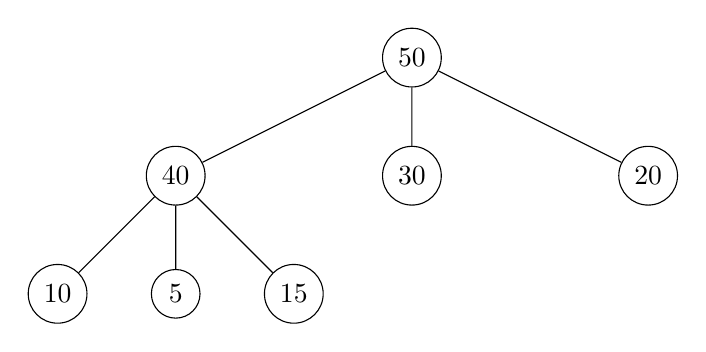
\begin{tikzpicture}[level/.style={sibling distance=3cm/#1, level distance=1.5cm}]
                    \node[circle,draw](50){50}
                      child{node[circle,draw]{40}
                        child{node[circle,draw]{10}}
                        child{node[circle,draw]{5}}
                        child{node[circle,draw]{15}}
                      }
                      child{node[circle,draw]{30}}
                      child{node[circle,draw]{20}};
                \end{tikzpicture}
            \end{center}


                \newpage
                
                \begin{bclogo}[logo={
\includegraphics[height=4ex]{Python-logo-notext.svg.png}}, noborder=true, couleur=white]{D-Ary Heap}
                    \begin{minted}{Python}
                        class DaryHeap:
                            def __init__(self, d):
                                self.d = d
                                self.heap = []
                        
                            def parent(self, i):
                                return (i - 1) // self.d
                        
                            def child(self, i, j):
                                return self.d * i + j + 1
                        
                            def insert(self, key):
                                self.heap.append(key)
                                i = len(self.heap) - 1
                                while i != 0 and self.heap[i] > self.heap[self.parent(i)]:
                                    self.heap[i], self.heap[self.parent(i)] = self.heap[self.parent(i)], self.heap[i]
                                    i = self.parent(i)
                        
                            def delete(self):
                                if len(self.heap) == 0:
                                    raise IndexError("Heap is empty")
                                max_val = self.heap[0]
                                last_val = self.heap.pop()
                                if len(self.heap) > 0:
                                    self.heap[0] = last_val
                                    self.heapify(0)
                                return max_val
                                
                            def heapify(self, i):
                                largest = i
                                for j in range(self.d):
                                    c = self.child(i, j)
                                    if c < len(self.heap) and self.heap[c] > self.heap[largest]:
                                        largest = c
                                if largest != i:
                                    self.heap[i], self.heap[largest] = self.heap[largest], self.heap[i]
                                    self.heapify(largest)
                    \end{minted}
                \end{bclogo}
    \section{Sorting Algorithms as Special Cases of a Priority Queue Sort}
        Dans "Sorting Algorithms as Special Cases of a Priority Queue Sort", Tim Bell introduit le concept de d-heap, qui est une généralisation de la structure de données du tas binaire. Un tas d est une structure de données arborescente où chaque nœud a jusqu'à d enfants, et la priorité de chaque nœud est supérieure ou égale à la priorité de ses enfants.

        Bell soutient que de nombreux algorithmes de tri peuvent être considérés comme des cas particuliers d'un tri de file d'attente prioritaire utilisant un d-heap. Plus précisément, il montre comment utiliser un d-heap pour implémenter le tri en tas, le tri en douceur et le tri par patience. Il présente également un nouvel algorithme de tri appelé d-heapsort, qui est une généralisation du tri en tas qui utilise un d-heap au lieu d'un tas binaire.

        L'article comprend également une analyse détaillée des caractéristiques de performance des algorithmes de tri basés sur d-heap, y compris la complexité temporelle et spatiale. Bell montre que le tri en tas a la même complexité temporelle que le tri en tas $ ( O ( n \log n )$ dans les cas moyens et les pires), mais peut avoir une meilleure complexité spatiale pour certaines valeurs de d .

        Dans l'ensemble, "Sorting Algorithms as Special Cases of a Priority Queue Sort" est une ressource utile pour ceux qui s'intéressent à la théorie et à la pratique des algorithmes de tri, et offre une nouvelle perspective sur la relation entre les files d'attente prioritaires et les algorithmes de tri.\footnote{AI generated.}

        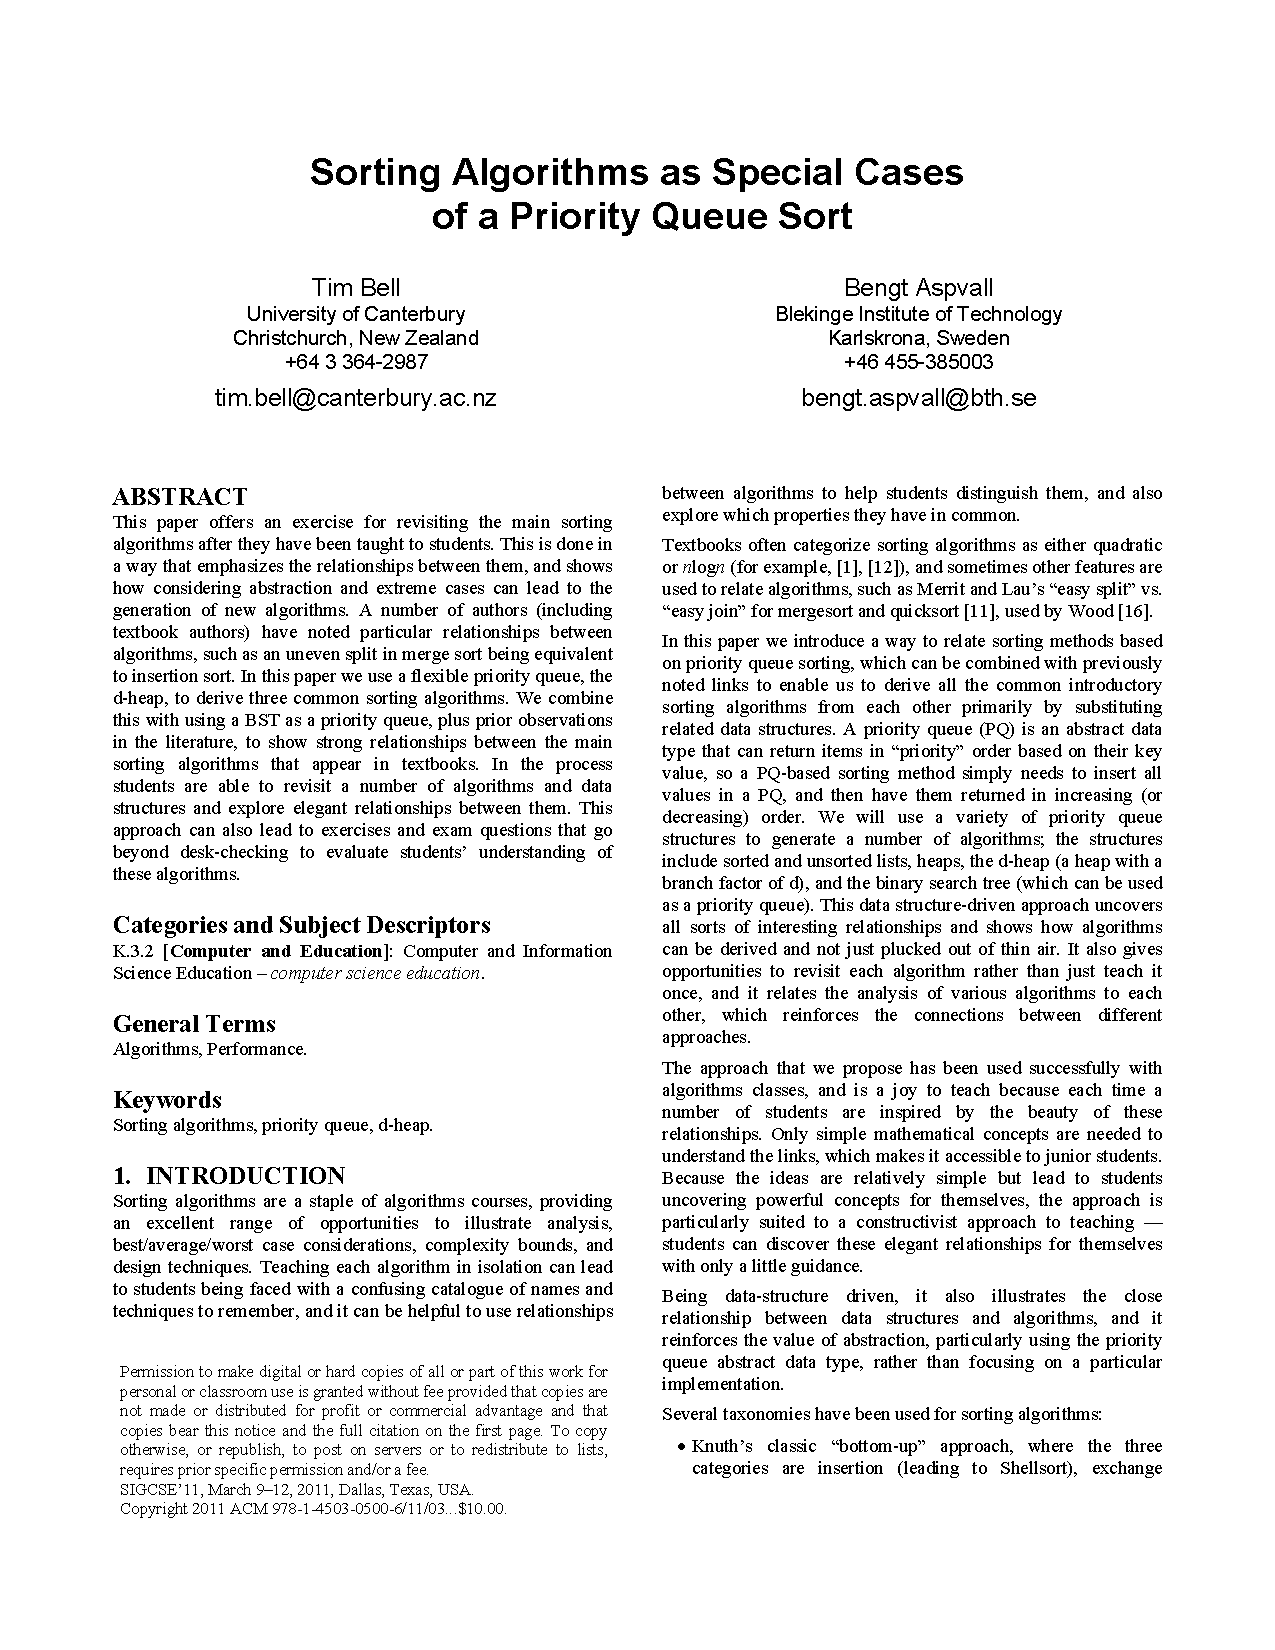
\includepdf[pages=-]{Bell Aspvall 2011 SIGCSE.pdf}

        \newpage 

        \subsection{Un peu de Python...}
            \begin{bclogo}[logo={
\includegraphics[height=4ex]{Python-logo-notext.svg.png}}, noborder=true, couleur=white]{Application d'Algortihme}
                \begin{minted}{Python}
                    def parent(i, d):
                        """
                        Returns the index of the parent of node i in a d-heap.
                        """
                        return (i - 1) // d
                    
                    def child(i, j, d):
                        """
                        Returns the jth child of node i in a d-heap.
                        """
                        return d * i + j + 1
                    
                    def max_heapify(A, i, n, d):
                        """
                        Maintains the max-heap property of a d-heap.
                        """
                        largest = i
                        for j in range(d):
                            c = child(i, j, d)
                            if c < n and A[c] > A[largest]:
                                largest = c
                        if largest != i:
                            A[i], A[largest] = A[largest], A[i]
                            max_heapify(A, largest, n, d)
                    
                    def build_max_dheap(A, d):
                        """
                        Builds a max d-heap from an array A in O(n) time.
                        """
                        n = len(A)
                        for i in range(n // d - 1, -1, -1):
                            max_heapify(A, i, n, d)
                    
                    def d_heapsort(A, d):
                        """
                        Sorts an array A using d-heapsort in O(n log n) time.
                        """
                        build_max_dheap(A, d)
                        n = len(A)
                        for i in range(n - 1, 0, -1):
                            A[0], A[i] = A[i], A[0]
                            max_heapify(A, 0, i, d)
                    
                \end{minted}
                \begin{minted}{Python}
                    A = [4, 1, 3, 2, 16, 9, 10, 14, 8, 7]
                    d = 3
                    d_heapsort(A, d)
                    print(A)
                \end{minted}
            \end{bclogo}
        
\end{document}          